%-----------------------------------------------------------------------
% 
%-----------------------------------------------------------------------
%
%     
%
%
%%%%%%%%%%%%%%%%%%%%%%%%%%%%%%%%%%%%%%%%%%%%%%%%%%%%%%%%%%%%%%%%%%%%%%%%


\documentclass[twoside]{article}
\usepackage{amsmath,amsthm,amssymb,verbatim}

%     If your article includes graphics, uncomment this command.
\usepackage{graphicx}

%     If the article includes commutative diagrams, ...
%\usepackage[cmtip,all]{xy}

\usepackage{url}

\usepackage{fancyhdr}
\pagestyle{fancy}

\usepackage{cite}



\def\blfootnote{\xdef\@thefnmark{}\@footnotetext} 
\long\def\symbolfootnote[#1]#2{\begingroup%
\def\thefootnote{\fnsymbol{footnote}}\footnote[#1]{#2}\endgroup} 

	\addtolength{\oddsidemargin}{1cm}
	\addtolength{\evensidemargin}{-1cm}

\setcounter{page}{1}

\begin{document}

%     If you need symbols beyond the basic set, uncomment this command.
%\usepackage{amssymb}


\newtheorem{theorem}{Theorem}[section]
\newtheorem{lemma}[theorem]{Lemma}

\theoremstyle{definition}
\newtheorem{definition}[theorem]{Definition}
\newtheorem{example}[theorem]{Example}
\newtheorem{xca}[theorem]{Exercise}

\theoremstyle{remark}
\newtheorem{remark}[theorem]{Remark}

\numberwithin{equation}{section}


\date{}
\lhead[]{}
\chead[\underline{Universality }]{\it{O. Shanker}}
\rhead[]{}

% \title[short text for running head]{full title}
\title{\bf{Universality of Riemann Zeta Function value distribution on critical axis}}

\maketitle


%    author one information
% \author[short version for running head]{name for top of paper}
\author{{\textbf{O. Shanker}},}
\thanks{ Mountain View, CA 94041, U. S. A. email: oshanker@gmail.com}

\thispagestyle{fancy}

%    Abstract is required.
\begin{abstract}
The behaviour of the Riemann zeta function, through its connections with
the spectra of random matrix theories and the spectra of classically 
chaotic quantum systems, is of enduring interest to 
statistical physics and condensed matter physics. Motivated by this unexpected and 
deep connection, we investigated
the value distribution of the Riemann zeta function on the critical axis.
We present a remarkable and striking universality property for the value distribution. 
The observed coefficients 
in the universality relation imply
symmetry and anti-symmetry relations for the value distribution.
We provide empirical verification of the relations for a range of heights along the critical
axis covering $16$ orders of magnitude. We discuss how random matrix models may shed further
light on this fundamental relation.

\end{abstract}
{\textbf {Keywords}:} Riemann zeta, Value Distribution, Universality, Symmetry, Hardy's function
\\
%{\textbf {PACS numbers}:}  02.70.Rr, 05.45.Df, 05.45.Pq


%\symbolfootnote[0]{\bf{* }}

%christopher.hughes@york.ac.uk https://arxiv.org/pdf/1911.03190.pdf

\section{Introduction}
Theoretical physicists studying statistical physics and condensed matter physics have a 
deep and enduring interest in the behaviour of the 
Riemann zeta function on the critical axis~\cite{Shanker 2006}. This is because of
its close and unusual connection  to the theory of the spectra of random matrix theories 
(RMT)~\cite{Wigner 1967, Gaudin 1960, Gaudin 1961, Dyson 1962, Bogomolny 1995, Bogomolny 1996, Katz 1999, Keating 2000a, Keating 2000b, Conrey 2000, 
Hughes 2000, Hughes 2001, Conrey 2002, Conrey 2003} 
and the spectra of classically chaotic quantum systems in 
physics~\cite{Berry 1985,Berry 1986,Berry 1987,Berry 1988}. Schumayer and
Hutchinson~\cite{Schumayer 2011} give a comprehensive review of the role
of the Riemann Hypothesis in several areas of physics, including condensed matter
and statistical physics. To get some insight into this, 
we look at the symmetry and universality properties of the Riemann zeta function value 
on the critical axis. This provides a complementary way to look at the problem.
The universality relations and symmetries exhibited by a system are fundamental aspects 
of the system. We discuss how random matrix models can be used to gain further insight
into the fundamental universal and symmetry properties.

Ref.~\cite{Shanker 2018a} studied empirically the distribution of $Z(t)$ values at 
Gram points and
showed  that the distribution for even Gram points was the negative  of the 
distribution for odd Gram points. 
Further work~\cite{Shanker 2018b}) extended the study to Generalized Gram points. 
The new results in this work are as follows. 
Our new universality relation (Eq.~\ref{eq:universality}) expresses the value distributions 
at different Generalized Gram points, in terms of three universal functions.
By universal we mean that the universal functions are independent of the angle $\phi$
characterizing the  Generalized Gram point.
We show that the  value
distribution of the Hardy $Z$ function at discrete points is anti-symmetrical 
for reflections around the mid-points 
of the Gram intervals (Eq.~\ref{eq:rhoantisym}) and symmetrical for reflections 
around the Gram points(Eq.~\ref{eq:rhosym}). 

Section~\ref{sec2} establishes the required notation for the 
Riemann Zeta Function. 
Section~\ref{sec3} presents the conjectured universality and symmetry relations
and provides evidence for the universality relations. We discuss the application
of random matrix theory to understand these fundamental properties.
In Section~\ref{sec4} we discuss the evidence for the symmetry relations
by studying the quantiles of the distributions.
Section~\ref{conclusions} presents the conclusions. 


\begin{figure*}
\centering
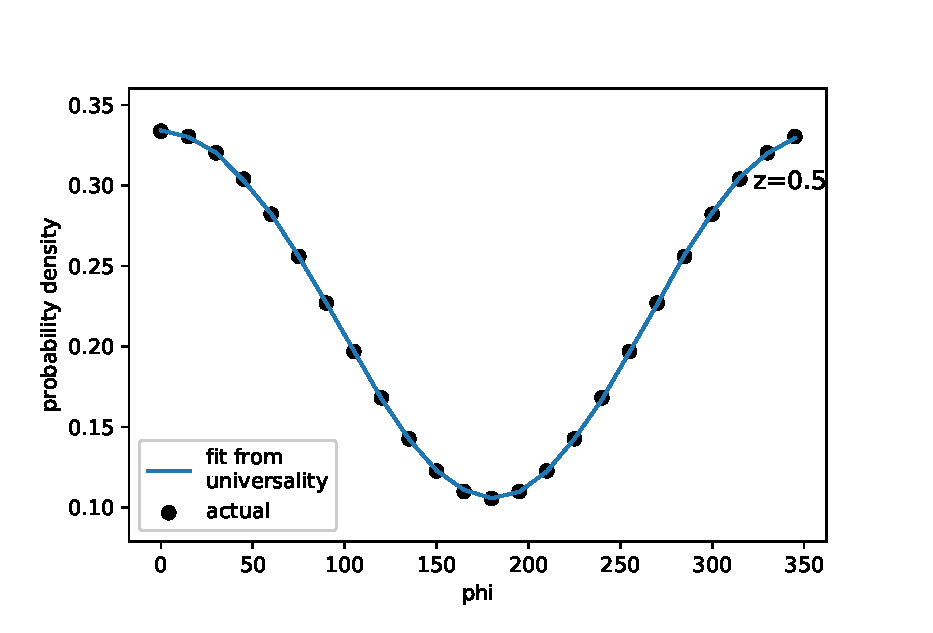
\includegraphics[width=0.8\textwidth]{z05.eps}
\caption[]{ 
 Test of universality. Comparison of probability density prediction from
 universality with actual values, for $z=0.5$. The y axis is the probability density.
 The x axis is the angle characterizing the Generalized Gram point.
  }
\vspace{1mm}
\label{z05}
\end{figure*}

\begin{figure*}
\centering
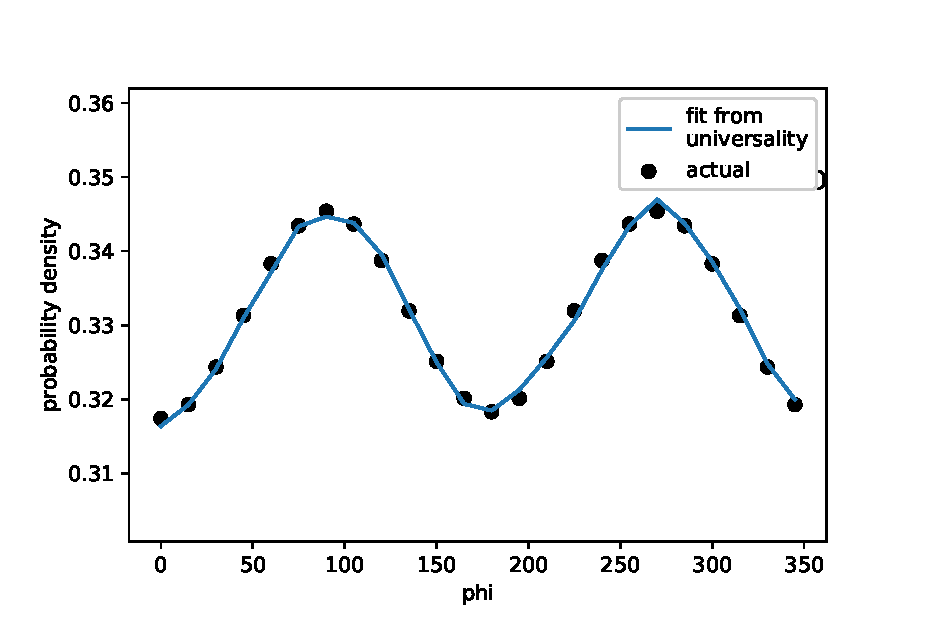
\includegraphics[width=0.8\textwidth]{z00.eps}
\caption[]{ 
 Test of universality. Comparison of probability density prediction from
 universality with actual values, for $z=0.0$. 
  }
\vspace{1mm}
\label{z00}
\end{figure*}

\section{\label{sec2}Notation for the Riemann zeta function}

In this section we  establish the required notation for the 
Riemann Zeta Function. 
For $\mathrm{Re} (s) > 1$ the Riemann Zeta function is defined as
\begin{equation}
\zeta ( s ) \, = \, \sum^{\infty}_{n = 1} \; n^{-s} \, = \, \prod_{p \in primes} \;
\left( 1 - p^{-s} \right)^{-1}.
\label{eqRie}
\end{equation}
 $\zeta ( s )$ can be continued to
the complex plane. Riemann's hypothesis, that the non-trivial zeros of $\zeta ( s )$ lie on the 
critical axis $1/2+it$, is probably the most famous unsolved problem in mathematics.
The mean spacing $\delta$ of the zeros  at large height $T$ is $\delta = 2\pi(\ln (T/2\pi))^{-1}$. 
For numerical studies of the Riemann hypothesis one defines Hardy's function
\begin{equation}
Z(t)=exp(i\theta(t))\zeta(1/2 +it) 
\label{eq:hardy}
\end{equation}
where 
\begin{equation}
\theta(t) = arg (\pi^{it/2} \Gamma(\frac{1}{4} + \frac{it}{2})). 
\label{eq:theta}
\end{equation}
The argument in Eq.~\ref{eq:theta} is defined by continuous variation of $t$ starting with the value $0$ at $t = 0$.
$Z(t)$ is real valued for real $t$,
and we have $|Z(t)| = |\zeta(1/2+it)|$. Thus the zeros of $Z(t)$ are the imaginary part of the zeros 
of $\zeta(s)$ which lie on the critical line.  

Gram points~\cite{Gram 1903} play an important role in the the theory because many of the zeros are separated by them.  When $t \ge 7$, the $\theta$ function Eq.(\ref{eq:theta}) is monotonic increasing. 
For $n \ge -1$, the $n$-th Gram point $g_n$ is defined as the unique solution $> 7$ to
$\theta (g_n) = n\pi$. A Gram interval is the interval $G_n = [g_n,g_{n+1})$.
 In analogy with Gram points, we can associate an angle $\phi$ with a point $t$ on the critical axis as follows:
\begin{definition}\label{phi}
For $t \ge 7$, $t$ is said to be a generalized Gram point with value $\phi$  if
$\theta (t) = 2k\pi + \phi$, where $0 \le \phi < 2\pi$.
\end{definition}



\section{\label{sec3}Universality and symmetry relations}

\begin{table}
\centering \(\begin{array}{ccccccc}
\hline
     z     & A   &      B      &   C    &R^2\\
\hline
-3.00& -0.028&  0.001&  0.039& 0.99982\\
  -2.50& -0.036&  0.001&  0.051& 0.99973\\
  -2.00& -0.047&  0.001&  0.068& 0.99988\\
  -1.50& -0.063&  0.001&  0.095& 0.99981\\
  -1.00& -0.086& -0.000&  0.140& 0.99991\\
  -0.50& -0.115& -0.004&  0.223& 0.99993\\
   0.00& -0.000& -0.014&  0.332& 0.99403\\
   0.50&  0.114& -0.004&  0.223& 0.99994\\
   1.00&  0.086&  0.000&  0.140& 0.99992\\
   1.50&  0.062&  0.001&  0.095& 0.99989\\
   2.00&  0.047&  0.001&  0.068& 0.99989\\
   2.50&  0.036&  0.001&  0.051& 0.99970\\
   3.00&  0.029&  0.001&  0.039& 0.99982\\
\hline
\end{array}\)
\caption{Values of the universal functions $A(z)$, $B(z)$ and $C(z)$ 
for $z$ in the range $-3.0$ to $3.0$, and the $R^2$ from the fit to actual values.} 
\label{tab:coefficients}
\end{table}

In this section we present the probability distribution function for the Riemann zeta function
values at Generalized Gram points. We present a universality relation satisfied by these distributions.

The sample space for our study is the interval along the critical axis specified by $(T_1, T_2)$. 
While empirical studies necessarily use large but finite  $T_1, T_2$, we are interested in the limit 
$T_1 \rightarrow \infty, T_2 \rightarrow \infty,  T_2-T_1 \rightarrow \infty,$ however
\begin{equation}
T_2 - T_1  \ll T_1. 
\label{eq:inter}
\end{equation}
Because of Equation~\ref{eq:inter}, we can consider  $\ln (t)$  to be effectively constant over  the interval.
The latter condition is not essential but is convenient, in that it simplifies the numerical work. 
The notation $\ln (t)$ stands for the natural logarithm of $t$.  
We study the probability distribution function for $Z(t)$ at generalized Gram  points,
 $p_{\phi}(y)$:
\begin{definition}\label{pphi}
\begin{equation}
\int\limits_{a}^{b} p_{\phi}(z)dz
\label{eq:pdfphi}
\end{equation}
is the probability that $a<Z(t)<b$ when we consider the values of $Z(t)$ for a large number of 
generalized Gram points in the sample space. 
\end{definition}
The probability density  $p_{\phi}(z)$ depends on the sample space (i.e., on the height $t$ and on the size of 
the sample space). In practice the densities are not sensitive to the choice of the sample space as long as 
the height $t$ is large enough and the length of the interval from which the sample is collected is large enough 
(but not too large on log scale). The  study of 
Kalpokas and Steuding \cite{kalpokas 2009} implies that the standard deviation of $p_{\phi}(z)$  
is independent of $\phi$ and is proportional to $\frac{T}{2\pi}$.  
The probability distribution will have a finite standard deviation if the 
argument is normalized by $\sqrt{\frac{T}{2\pi}}$.

\begin{table}
\centering \(\begin{array}{ccccccccccc}

\hline
\phi  &  \multicolumn{2}{c}  {0 }   &    \multicolumn{2}{c}  {\pi/6}&  \multicolumn{2}{c}  { \pi/4}   &    \multicolumn{2}{c}  {\pi/3}&  \multicolumn{2}{c}  {\pi/2 } \\
z&actual&predict&actual&predict &actual&predict &actual&predict &actual&predict\\
\hline
  -3.00&  0.012&  0.012&  0.016&  0.015&  0.019&  0.019&  0.025&  0.024&  0.038&  0.038 \\
  -2.50&  0.016&  0.016&  0.020&  0.020&  0.025&  0.025&  0.032&  0.032&  0.050&  0.050 \\
  -2.00&  0.023&  0.022&  0.028&  0.028&  0.035&  0.035&  0.044&  0.044&  0.067&  0.067 \\
  -1.50&  0.033&  0.033&  0.041&  0.041&  0.050&  0.051&  0.063&  0.063&  0.094&  0.094 \\
  -1.00&  0.054&  0.054&  0.065&  0.066&  0.079&  0.080&  0.098&  0.097&  0.140&  0.140 \\
  -0.50&  0.105&  0.105&  0.122&  0.122&  0.143&  0.142&  0.167&  0.168&  0.227&  0.227 \\
   0.00&  0.316&  0.317&  0.324&  0.324&  0.331&  0.331&  0.337&  0.338&  0.345&  0.345 \\
   0.50&  0.334&  0.334&  0.320&  0.320&  0.303&  0.304&  0.282&  0.282&  0.227&  0.227 \\
   1.00&  0.227&  0.226&  0.213&  0.214&  0.200&  0.201&  0.183&  0.183&  0.140&  0.140 \\
   1.50&  0.157&  0.158&  0.149&  0.150&  0.140&  0.139&  0.127&  0.126&  0.093&  0.095 \\
   2.00&  0.115&  0.115&  0.109&  0.109&  0.101&  0.101&  0.091&  0.091&  0.068&  0.067 \\
   2.50&  0.088&  0.088&  0.083&  0.083&  0.077&  0.076&  0.068&  0.069&  0.050&  0.050 \\
   3.00&  0.069&  0.069&  0.065&  0.064&  0.059&  0.060&  0.054&  0.053&  0.039&  0.039 \\
\hline
\end{array}\)
\caption{Comparison of actual and predicted probability density for some $\phi$   }
\label{tab:pred}
\end{table}



The universality relation is
\begin{equation}
p_{\phi}(z) = A(z)\cos(\phi) + B(z)\cos(2\phi) +C(z),
\label{eq:universality}
\end{equation}
where $A(z)$, $B(z)$ and $C(z)$ are universal functions, i.e., they do not depend on $\phi$. 
The anti-symmetry relation is
\begin{equation}
p_{\phi}(z) = p_{\phi+\pi}(-z).
\label{eq:rhoantisym}
\end{equation}
The symmetry relation is
\begin{equation}
p_{\phi}(z) = p_{2\pi-\phi}(z).
\label{eq:rhosym}
\end{equation}

We estimated $A(z)$, $B(z)$ and $C(z)$ by fitting Eq.~\ref{eq:universality} to the actual
probability densities for several values of $z$ and $\phi$. Table~\ref{tab:coefficients} gives the 
fitted values 
of the universal functions.
Fig~\ref{z05} and Fig.~\ref{z00} and Table~\ref{tab:pred} show the comparison of the predictions 
from the universality 
relation to the actual probability densities, for some values of the argument $z$.
The figures, and 
Table~\ref{tab:pred} show the excellent agreement of the actual probability densities with the
universality relations prediction. 
From the symmetry relations Eq.~\ref{eq:rhosym} and Eq.~\ref{eq:rhosym} we find 
that the function 
$A(z)$ has to be anti-symmetric in $z$, and $B(z)$ and $C(z)$ have to be symmetric in $z$.
Table~\ref{tab:coefficients} confirms these properties. 
The mean value of $z$ is known from theory to be $2\cos(\phi)$~\cite{Shanker 2018b}. 
Eq.~\ref{eq:universality} gives an understanding of why the mean value is proportional to 
$\cos(\phi)$.

Since the $A(z)$, $B(z)$ and $C(z)$ show large variation close to $z=0.0$, we plot
these functions for this region. Fig~\ref{Az}, Fig~\ref{Bz} and Fig~\ref{Cz} 
show the variation.


\begin{figure*}
\centering
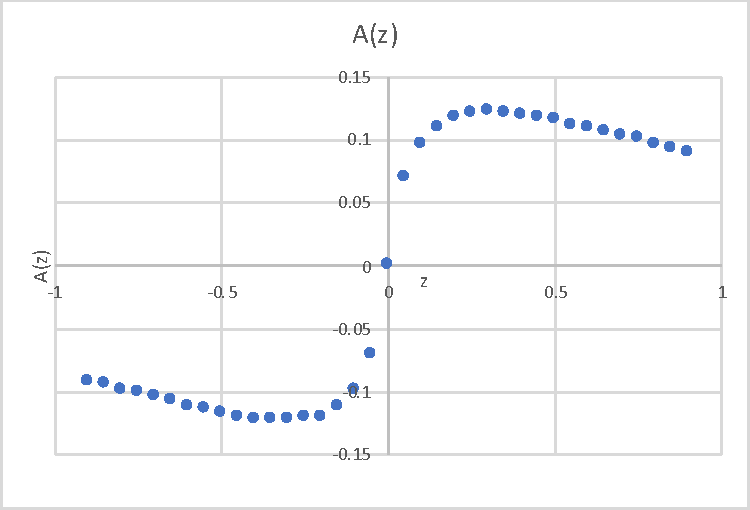
\includegraphics[width=0.8\textwidth]{Az.pdf}
\caption[]{ 
 Plot of $A(z)$ around $z=0.0$. 
  }
\vspace{1mm}
\label{Az}
\end{figure*}

\begin{figure*}
\centering
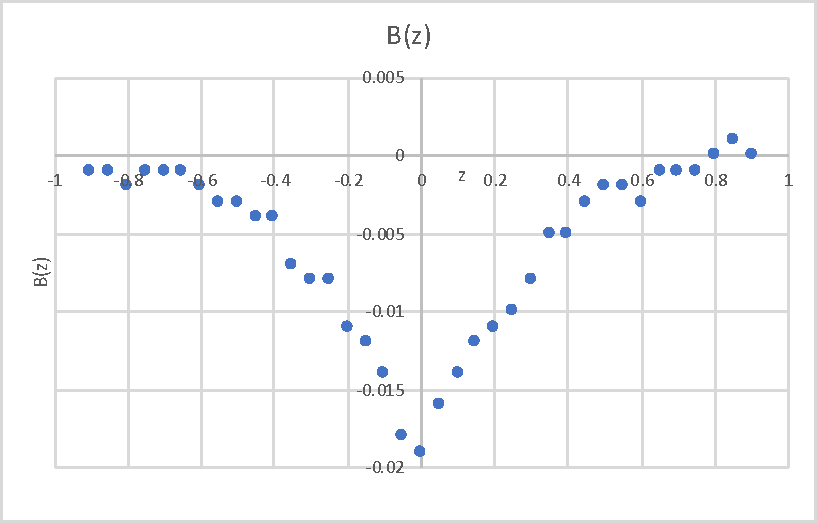
\includegraphics[width=0.8\textwidth]{Bz.pdf}
\caption[]{ 
 Plot of $B(z)$ around $z=0.0$. 
  }
\vspace{1mm}
\label{Bz}
\end{figure*}

\begin{figure*}
\centering
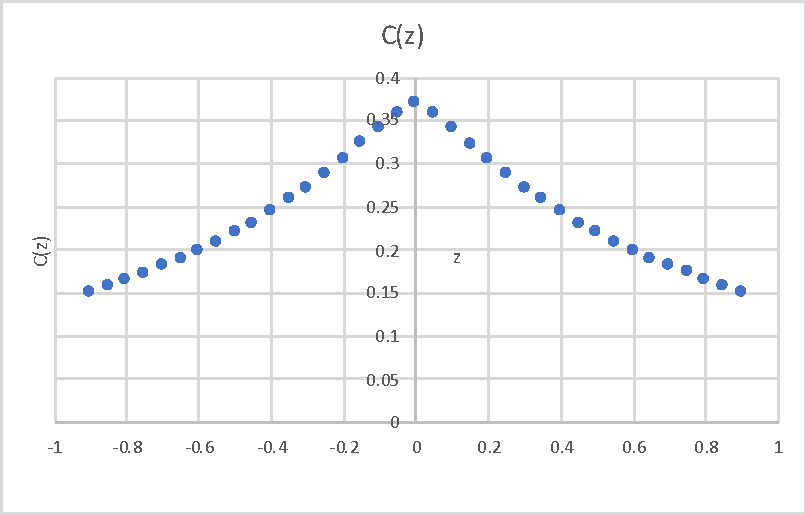
\includegraphics[width=0.8\textwidth]{Cz.pdf}
\caption[]{ 
 Plot of $C(z)$ around $z=0.0$. 
  }
\vspace{1mm}
\label{Cz}
\end{figure*}


\subsection{\label{related}Random matrix models}
A possible fruitful avenue of future investigation may be to relate the distributions to 
the results of Random Matrix Theory (RMT).  Keating and  Snaith~\cite{Keating 2000a} introduced the 
characteristic polynomial of a unitary matrix as a RMT model for the Riemann zeta function. 
Let $U(N)$ be the group of  all $N \times N$ unitary matrices.
If $A \in U(N)$, the characteristic polynomial $P(\theta)$ is defined as
\begin{equation}
P(\theta) = det(I_N-A\exp {(i\theta)}),
\label{eq:uNeigen}
\end{equation}
where $det$ is the determinant, and $I_N$ is the unit matrix.
Hanga and Hughes~\cite{Hanga 2020} define Gram points for  $U(N)$ and 
for $SU(N)$, the group of 
all $N \times N$ special unitary matrices. They show that the $SU(N)$ group gives
a better approximation to the distribution of zeros in Gram intervals, for large but
finite $N$. It will be useful to push these results further, and maybe define 
generalized Gram points for these groups.

Ivi\'c's monograph~\cite{Ivic 2013} 
has a comprehensive survey of  the  closely related Hardy's function~\cite{Hardy 1918}.
Selberg in unpublished work showed that at large $t$ $\log (\zeta(\frac{1}{2} + it))$ is 
approximately normally distributed with a standard deviation of 
order $\sqrt{log~log~t}$ (see Ref.~\cite{Hejhal}). He showed a 
similar result~\cite{Selberg 1989, Selberg 1991} for $\log (|Z(t)|)$. 
Laurincikas~\cite{Laurincikas}  used probabilistic number theory to prove various results 
about the distribution of the Riemann zeta function.

Regarding the value distribution at specific points along the Gram interval, 
Titchmarsh~\cite{Titchmarsh 1934} and Kalpokas and Steuding~\cite{kalpokas 2009} present 
results pertaining to the
mean value of the Riemann zeta function. Lester's~\cite{Lester 2013} Ph. D. thesis also 
considers the distribution of $\log (|\zeta(\frac{1}{2} + it)|)$  for specific points along the Gram interval.  
The question of the values of Hardy's $Z$-function at a discrete sequence of points on the critical axis 
is quite interesting. The above references give some results in this direction that can be proved rigorously. 
At the same time, the present state of Riemann zeta function theory gives limited information 
about the value distribution of $Z(t)$ at discrete sequences of points. Possibly, these analogues 
could differ significantly from the continuous case.  
Our numerical studies of the value distribution of Hardy's $Z$-function at discrete points
helps fill the gaps. 


\subsection{\label{numerics}Numerical evaluation}


We evaluate Hardy's function $Z(t)$  using the Riemann$-$Siegel series
\begin{equation}
Z(t) = 2\sum^{m}_{n=1}\frac{\cos(\theta(t) - t \ln (n))}{\sqrt{n}} + R(t), 
\label{eq:RS}
\end{equation}
where $m$ is the integer part of $\sqrt{t/(2\pi)}$. $R(t)$ is a small remainder
term which can be evaluated to the desired level of accuracy. We used the techniques in
 Refs.~\cite{Odlyzko 1992,hiary,gourdon} 
to efficiently evaluate the zeta function at large $t$. To evaluate  $Z(t)$  at several points 
in the Gram interval, we have to use band limited function interpolation~\cite{Jerri 1977}. 
We evaluate the coefficients in the series for band limited function interpolation at the Gram points, 
and use the series to evaluate $Z(t)$ at other points in the Gram interval. The most important 
source for loss of accuracy at large heights is the cancellation between
large numbers that occur in the arguments of the $\cos$ terms in Eq.~(\ref{eq:RS}). We 
use a high precision module to evaluate the arguments. The rest of the calculation
is done using regular double precision accuracy. The  zeros from Ref~\cite{hiary 2010} 
were used 
to check the accuracy of our zeta function calculations. 
Our evaluations of $Z(t)$ at $T=10^{12}$ 
are accurate 
to better than $10^{-6}$. 


\section{\label{sec4}Evidence for the relations from quantiles}
  
The human mind is attracted by symmetry. Many objects in nature exhibit symmetry.
Even more remarkable are the symmetries exhibited in the basic laws of the 
universe. In this section we present  numerical evidence for the symmetry properties
Eq.~\ref{eq:rhosym} and Eq.~\ref{eq:rhoantisym}. 
We  present the distribution for $T=10^{12}$, followed by the distribution for $T=10^{28}$.  
We are interested in how the symmetry properties behave when we span a large range of 
height $T$.
We will present the symmetry properties in terms of the quantiles~\cite{feller} 
for the sample space. This is because for any sample space the quantiles are well defined 
and always exist. We recall that in statistics, given a fraction $f$ between $0$ and $1$, 
the quantile $q_f$ is the value such that fraction $f$  of the sample population is 
at or below $q_f$. For example, $q_{0.5}$ is the median of the sample.
For $f$ very close to $0$ or $1$, in the limiting case $q_f$ will diverge. 
However we will assume that there is a range of $f$ for which well-defined limits exist. 
If necessary we can normalize the $Z$ values by some power of $\ln(T/2\pi)$ without 
affecting the symmetry properties. Since the standard deviation is 
known to be $sqrt(\ln(T/2\pi))$~\cite{Shanker 2018b}, 
normalizing $Z$ by this factor will make $q_f$ finite for finite $f$. 
Certainly, for our two samples separated by several orders of magnitude, 
we find that the quantile distribution changes very little. 

In terms of quantiles the anti-symmetry relation Eq.~\ref{eq:rhoantisym} 
can be written
\begin{equation}
q_{f}(\phi) = -q_{1-f}(\pi-\phi).
\label{eq:antisym}
\end{equation}
Eq.~\ref{eq:antisym}  is a generalization of the result in Ref.~\cite{Shanker 2018a} 
for the anti-symmetry of the distribution of $Z(t)$ at even and odd Gram points. 
The  symmetry condition Eq.~\ref{eq:rhosym} implies
\begin{equation}
q_{f}(\phi) = q_{f}(2\pi-\phi).
\label{eq:sym}
\end{equation}




\subsection{\label{E12}Quantiles for $Z(t)$ at $T=10^{12}$}


\begin{table}
\centering \(\begin{array}{cccccccccccc}

\hline
0&\pi/6 &\pi/3 &\pi/2 &2\pi/3 &5\pi/6 &\pi &7\pi/6 &4\pi/3 &3\pi/2 &5\pi/3 &11\pi/6 \\
2.000 &1.732 &1.000 &0.000 &-1.000 &-1.732 &-2.000 &-1.732 &-1.000 &0.000 &1.000 &1.732 \\
4.998&5.002&5.004&5.004&5.000&4.996&4.991&4.987&4.985&4.986&4.989&4.993 \\
\hline
\end{array}\)
\caption{Mean    $Z(t)$ and Standard Deviation at $T=10^{12}$. Row 1: $\phi$, Row 2: mean~$Z$, Row 3: Standard Deviation}
\label{tab:mean12}
\end{table}

\begin{table}
\centering \(\begin{array}{cccccccccccc}
\hline
\phi&0.1&0.2&0.25&0.3&0.4&0.5&0.6&0.7&0.75&0.8&0.9 \\
\hline
0&-0.687&-0.011&0.113&0.234&0.506&0.852&1.324&2.031&2.54&3.229&5.876\\
\pi/6 &-1.055&-0.161&0.017&0.138&0.401&0.732&1.188&1.865&2.352&3.008&5.577\\
\pi/3 &-2.068&-0.709&-0.388&-0.164&0.123&0.411&0.801&1.39&1.815&2.4&4.688\\
\pi/2 &-3.415&-1.543&-1.082&-0.75&-0.297&0.002&0.299&0.753&1.089&1.555&3.415\\
2\pi/3 &-4.693&-2.391&-1.81&-1.382&-0.795&-0.405&-0.119&0.165&0.39&0.713&2.068\\
5\pi/6 &-5.586&-3.006&-2.338&-1.852&-1.178&-0.726&-0.396&-0.137&-0.016&0.162&1.051\\
\pi &-5.9&-3.218&-2.528&-2.024&-1.319&-0.847&-0.503&-0.231&-0.112&0.012&0.687\\
7\pi/6 &-5.569&-2.995&-2.334&-1.851&-1.182&-0.729&-0.399&-0.137&-0.016&0.163&1.048\\
4\pi/3 &-4.674&-2.387&-1.803&-1.379&-0.799&-0.41&-0.123&0.166&0.388&0.712&2.066\\
3\pi/2 &-3.407&-1.543&-1.083&-0.75&-0.296&-0.001&0.297&0.751&1.084&1.549&3.403\\
5\pi/3 &-2.061&-0.705&-0.386&-0.164&0.122&0.409&0.797&1.384&1.81&2.391&4.67\\
11\pi/6 &-1.037&-0.159&0.018&0.14&0.4&0.732&1.183&1.851&2.339&3.004&5.56\\

\hline
\end{array}\)
\caption{Quantiles  for  $Z(t)$ at $T=10^{12}$.}
\label{tab:quantiles12}
\end{table}


\begin{table}
\centering \(\begin{array}{cccccccccccc}
\hline
$f$&0.1&0.2&0.25&0.3&0.4&0.5&0.6&0.7&0.75&0.8&0.9\\
\hline
intercept&-3.346&-1.569&-1.134&-0.817&-0.360&0.002&0.362&0.821&1.139&1.575&3.342\\
slope&1.307&0.817&0.678&0.577&0.457&0.420&0.457&0.578&0.681&0.819&1.302\\
R^2&0.999&0.999&0.997&0.995&0.996&1.000&0.996&0.995&0.997&0.999&0.999\\
\hline
\end{array}\)
\caption{Linear fit of quantile $q_f$ to $2\cos(\phi)$ at $T=10^{12}$.}
\label{tab:fit12}
\end{table}

Table~\ref{tab:mean12} shows the mean value for $Z(T)$ and the standard deviation at $12$ equally spaced values 
of $\phi$ at $T=10^{12}$. 
The mean value is known from theory to be $2\cos(\phi)$, and the standard deviation is known 
to be $sqrt(\ln(T/2\pi))$~\cite{Shanker 2018b}. The table verifies this result to better 
than one part in a thousand. Table~\ref{tab:quantiles12} shows the quantiles for $Z(T)$. 
Eq.~\ref{eq:antisym} can be verified, for example, by noting that $q_f$ in Table~\ref{tab:quantiles12}
for $\phi=\pi/6$ and $f=0.25$ is $0.017$, while it is $-0.016$ for $\phi=5\pi/6$ and $f=0.75$. 
Eq.~\ref{eq:sym} can be verified, for example, by noting that $q_f$ is $0.018$ for $\phi=11\pi/6$ and $f=0.25$.

We found that there is a linear dependence of the quantiles on $\cos(\phi)$. 
Table~\ref{tab:fit12} shows the intercept and slope when $q_f$ for any $f$ is fitted to
$2\cos(\phi))$. The observation of this relation itself verifies the symmetry condition 
Eq.~\ref{eq:sym} (i.e., there is no dependence on $\sin(\phi)$). 
The anti-symmetry condition Eq.~\ref{eq:antisym} implies that the intercept is anti-symmetric 
for reflection around $f=0.5$, while the slope is symmetric for such a reflection. This can be verified from the table. Table~\ref{tab:fit12} makes the symmetry and anti-symmetry relations stand out clearly.  It must be pointed out that Eq.~\ref{eq:antisym} and Eq.~\ref{eq:sym} do not require the
existence of the linear relationship of $q_f$ to $\cos(\phi)$. However, the linear relationship is consistent with the symmetry relations.
The linear dependence and the symmetry properties imply that the quartile range $q_{1-f}-q_f$ is independent of $\phi$.

\begin{table}
\centering \(\begin{array}{cccccccccccc}

\hline
0&\pi/6 &\pi/3 &\pi/2 &2\pi/3 &5\pi/6 &\pi &7\pi/6 &4\pi/3 &3\pi/2 &5\pi/3 &11\pi/6 \\
\hline
1.995&1.728&0.997&-0.002&-1.000&-1.731&-1.999&-1.731&-1.000&-0.002&0.997&1.728 \\
7.886&7.816&7.882&8.011&8.054&7.980&7.858&7.796&7.877&8.022&8.078&8.010 \\
\hline
\end{array}\)
\caption{Mean    $Z(t)$ and Standard Deviation at $T=10^{28}$. Row 1: $\phi$, Row 2: mean~$Z$, Row 3: Standard Deviation}
\label{tab:mean28}
\end{table}


\subsection{\label{E28}Quantiles for $Z(t)$ at $T=10^{28}$}

\begin{table}
\centering \(\begin{array}{cccccccccccc}
\hline
\phi&0.1&0.2&0.25&0.3&0.4&0.5&0.6&0.7&0.75&0.8&0.9 \\
\hline
0&-1.269&-0.220&-0.031&0.076&0.305&0.625&1.096&1.838&2.399&3.185&6.457\\
\pi/6 &-1.662&-0.388&-0.135&0.014&0.235&0.539&0.985&1.695&2.230&2.985&6.128\\
\pi/3 &-2.671&-0.896&-0.510&-0.257&0.042&0.294&0.674&1.288&1.756&2.424&5.269\\
\pi/2 &-4.028&-1.652&-1.112&-0.743&-0.272&0.001&0.271&0.743&1.115&1.651&4.003\\
2\pi/3 &-5.314&-2.433&-1.756&-1.284&-0.673&-0.296&-0.044&0.254&0.511&0.898&2.665\\
5\pi/6 &-6.214&-3.000&-2.232&-1.693&-0.977&-0.535&-0.233&-0.013&0.134&0.382&1.629\\
\pi &-6.524&-3.206&-2.407&-1.840&-1.088&-0.621&-0.302&-0.074&0.032&0.220&1.261\\
7\pi/6 &-6.220&-3.012&-2.237&-1.696&-0.982&-0.535&-0.232&-0.011&0.137&0.394&1.658\\
4\pi/3 &-5.314&-2.437&-1.763&-1.290&-0.669&-0.293&-0.042&0.254&0.512&0.898&2.660\\
3\pi/2 &-4.034&-1.659&-1.115&-0.743&-0.271&0.001&0.273&0.743&1.117&1.656&4.006\\
5\pi/3 &-2.689&-0.894&-0.510&-0.255&0.045&0.298&0.672&1.286&1.763&2.439&5.276\\
11\pi/6 &-1.642&-0.384&-0.133&0.013&0.233&0.534&0.977&1.691&2.229&2.990&6.152\\
\hline
\end{array}\)
\caption{Quantiles  for  $Z(t)$ at $T=10^{28}$.}
\label{tab:quantiles28}
\end{table}

\begin{table}
\centering \(\begin{array}{cccccccccccc}
\hline
$f$&0.1&0.2&0.25&0.3&0.4&0.5&0.6&0.7&0.75&0.8&0.9\\
\hline
intercept&-3.963&-1.680&-1.161&-0.807&-0.339&0.002&0.342&0.809&1.162&1.678&3.933\\
slope&1.318&0.757&0.606&0.493&0.351&0.308&0.352&0.492&0.604&0.751&1.302\\
R^2&0.999&0.999&0.998&0.994&0.993&1.000&0.992&0.994&0.998&1.000&0.999\\
\hline
\end{array}\)
\caption{Linear fit of quantile $q_f$ to $2\cos(\phi)$ at $T=10^{28}$.}
\label{tab:fit28}
\end{table}


To perform a rigorous test of the symmetry relations, we repeat the study for another $T$ separated from the first sample by $16$ orders of magnitude. At $T=10^{28}$ we used the  zeros from Ref~\cite{hiary 2010} to get the coefficients in the series for band limited function interpolation. We could then use this series to evaluate  $Z(t)$  at several points in the Gram interval.
Table~\ref{tab:mean28} shows the mean value for $Z(T)$  and the standard deviation at $12$ equally spaced values of $\phi$ at $T=10^{28}$. The table verifies that the values are $2\cos(\phi)$, to a few parts in a thousand. Table~\ref{tab:quantiles28} shows the quantiles for $Z(T)$.  Eq.~\ref{eq:antisym} can be verified, for example, by noting that $q_f$ in Table~\ref{tab:quantiles28}
for $\phi=\pi/6$ and $f=0.25$ is $-0.135$, while it is $0.134$ for $\phi=5\pi/6$ and $f=0.75$. Eq.~\ref{eq:sym} can be verified, for example, by noting that $q_f$ is $-0.133$ for $\phi=11\pi/6$ and $f=0.25$. Table~\ref{tab:fit28} verifies the linear relationship of $q_f$ to $\cos(\phi)$. The anti-symmetry condition Eq.~\ref{eq:antisym}  and the symmetry condition Eq.~\ref{eq:sym} are also verified in the table.


\section{\label{conclusions}Conclusions}

The most exciting new result is the discovery of a universality relation for the 
value distribution of the Hardy Z function at discrete points. Eq.~\ref{eq:universality}
states the universality relations. Table~\ref{tab:coefficients} gives the fitted values 
of the universal functions.
Fig~\ref{z05} and Fig.~\ref{z00} show the comparison of the predictions from the universality 
relation to the actual probability densities, for some values of the argument $z$. The figures, and 
Table~\ref{tab:pred} show the excellent agreement of the actual probability densities with the
universality relations prediction.
The evidence for the anti-symmetry and symmetry properties 
in terms of quantiles is illuminating. 
It is noteworthy that the quantile distributions change very little 
when the height $T$ spans $16$ orders of magnitude. 
Another intriguing observation is the linear dependence of the quantiles 
on $\cos(\phi)$. The linear dependence and the symmetry properties imply that 
the quartile range $q_{1-f}-q_f$ is independent of $\phi$.


\bibliographystyle{amsplain}
\begin{thebibliography}{10}

\bibitem{Shanker 2006} O. Shanker, 
``Random Matrices, Generalised Zeta Functions and Self-Similarity of Zero Distributions''
{\it J. Phys. A: Math. Gen.}, {\bf A 39}, 13983-13997, (2006). 

\bibitem{Wigner 1967} E. Wigner, “Random Matrices in Physics,” Siam Review, {\bf 9}, 1-23, (1967).
\bibitem{Gaudin 1960} M. Gaudin, M. Mehta, “On the Density of Eigenvalues of a Random Matrix,” 
Nucl. Phys., {\bf 18},
420-427, (1960).
\bibitem{Gaudin 1961} M. Gaudin, 
“Sur la loi Limite de L’espacement de Valuers Propres D’une Matrics Aleatiore,” 
Nucl. Phys., {\bf 25}, 447-458, (1961).
\bibitem{Dyson 1962} F. Dyson, “Statistical Theory of Energy Levels III,” 
J. Math. Phys., {\bf 3}, 166-175, (1962).

\bibitem{Bogomolny 1995} E.B. Bogomolny and J.P. Keating, Random matrix theory and the Riemann zeros I: three- and
four-point correlations, Nonlinearity, 8:1115–1131, 1995.
\bibitem{Bogomolny 1996} E.B. Bogomolny and J.P. Keating, Random matrix theory and the Riemann zeros II:n-point
correlations, Nonlinearity, 9:911–935, 1996.
\bibitem{Katz 1999} Nicholas M. Katz, Peter Sarnak, Random Matrices, Frobenius Eigenvalues and Monodromy, AMS,
Providence, Rhode Island, 1999.
\bibitem{Keating 2000a} J.P. Keating and N.C. Snaith, Random matrix theory and $\zeta(1/2 + it)$, 
Commun. Math. Phys., 214:57–89, 2000.
\bibitem{Keating 2000b} J.P. Keating and N.C. Snaith, Random matrix theory and L-functions at s = 1/2, 
Commun.
Math. Phys, 214:91–110, 2000.
\bibitem{Conrey 2000} J.B. Conrey and D.W. Farmer, Mean values of L-functions and symmetry, Int. Math. Res.
Notices, 17:883–908, 2000, arXiv:math.nt/9912107.
\bibitem{Hughes 2000} C.P. Hughes, J.P. Keating, and N. O’Connell, Random matrix theory and the derivative of the
Riemann zeta function, Proc. R. Soc. Lond. A, 456:2611–2627, 2000.
\bibitem{Hughes 2001} C.P. Hughes, J.P. Keating, and N. O’Connell, On the characteristic polynomial of a random
unitary matrix, Commun. Math. Phys., 220(2):429–451, 2001.
\bibitem{Conrey 2002} J.B. Conrey, D.W. Farmer, J.P. Keating, M.O. Rubinstein, and N.C. Snaith, Integral moments
of zeta- and L-functions, preprint, 2002, arXiv:math.nt/0206018.
\bibitem{Conrey 2003} J.B. Conrey, D.W. Farmer, J.P. Keating, M.O. Rubinstein, and N.C. Snaith, Autocorrelation of
Random Matrix Polynomials Commun. Math. Phys , 237:365-395, 2003

\bibitem{Berry 1985}  M. V. Berry, “Semiclassical theory of spectral rigidity,” 
Proc. R. Soc., {\bf A 400} , 229-251, (1985). 
\bibitem{Berry 1986}  M. V. Berry, “Riemann’s zeta function: a model for quantum chaos?,” 
Quantum chaos and
statistical nuclear physics (Springer Lecture Notes in Physics), {\bf 263}, 1-17, (1986).
\bibitem{Berry 1987}  M. V. Berry, “Quantum Chaology,” 
Proc. R. Soc. , A 413 , {\bf 183-198}, (1987).
\bibitem{Berry 1988}  M. V. Berry, ‘Number variance of the Riemann zeros‘,”
 NonLinearity , {\bf 1}, 399-407 , (1988).

\bibitem{Schumayer 2011} Daniel Schumayer and David A.W. Hutchinson,
"Physics of the Riemann Hypothesis"
{\it Rev.Mod.Phys.} {\bf83}, 307-330, (2011)

\bibitem{Shanker 2018a} O. Shanker, 
``Good to Bad Gram Point Ratio For Riemann Zeta Function",
{\it Experimental Mathematics} {\bf doi:10.1080/10586458.2018.1492474}(2018)

\bibitem{Shanker 2018b} O. Shanker, 
``Symmetry properties of distribution of Riemann Zeta Function values on critical axis''
{\it Advanced Modeling and Optimization}, {\bf 20}, 435-445, (2018). 

\bibitem{Gram 1903} J. P. Gram, 
``Sur les Zeros de la Fonction  $\zeta ( s )$  de Riemann",
{\it Acta Math.} {\bf27}(1903), 289-304



\bibitem{Hanga 2020} Catalin Hanga and Christopher Hughes,
"PROBABILISTIC MODELS FOR GRAM’S LAW", \url {https://arxiv.org/pdf/1911.03190.pdf}


\bibitem {Ivic 2013} Aleksandar Ivi\'c, ``The Theory of Hardy's Z-Function,''
Cambridge University Press,  (2013)

\bibitem{Hardy 1918} G. H. Hardy and J. E. Littlewood,
``Contributions to the theory of the Riemann
zeta-function and the distribution of primes",
{\it Acta Math.} {\bf41}(1918), 119-196

\bibitem{Hejhal} D. A. Hejhal,
``On a result of Selberg concerning zeros of linear combinations
of L-functions", 
{\it Int. Math. Res. Not.} {\bf11}(2000), 551-577

\bibitem {Selberg 1989} A. Selberg, ``Selected Papers, Vol. I,''
Springer Verlag,  (1989)

\bibitem {Selberg 1991} A. Selberg, ``Selected Papers, Vol. II,''
Springer Verlag,  (1991)



\bibitem{Laurincikas} A. Laurincikas,
``Limit Theorems for the Riemann Zeta-Function",
Kluwer, Dordrecht, 1996

\bibitem{Titchmarsh 1934} E. C. Titchmarsh,
``On van der Corput's method and the zeta-function of Riemann (IV)",
{\it Quart. J. Math. Oxford Ser.} {\bf5}(1934), 98-105

\bibitem{kalpokas 2009} J. Kalpokas and J. Steuding,
``On the value-distribution of the Riemann zeta-function on the critical line", 
{\it Moscow Journal of Combinatorics and
Number Theory} {\bf1}(2011), 26-42

\bibitem {Lester 2013} Stephen J. Lester, ``The Distribution of Values of the
Riemann Zeta-Function,''
Ph. D. dissertation, University of Rochester,  (2013)

\bibitem{Odlyzko 1992}  A. Odlyzko,
``The $10^{20}$-th Zero of the Riemann Zeta
Function and 175 Million of its Neighbors", report,
\url{http://www.dtc.umn.edu/~odlyzko/unpublished/zeta.10to20.1992.pdf}, (1992)

\bibitem{hiary} G. A. Hiary,
``Fast methods to compute the Riemann zeta function",
{\it Annals of Mathematics} {\bf174}(2011), 891-946

\bibitem{gourdon} Xavier Gourdon,
``The $10^{13}$ first zeros of the Riemann Zeta function,
and zeros computation at very large height", report,
\url{http://numbers.computation.free.fr/Constants/Miscellaneous/zetazeros1e13-1e24.pdf}, (2004)

\bibitem{Jerri 1977} A. J. Jerri,
``The Shannon sampling theorem - its various extensions and applications",
{\it Proc IEEE} {\bf65}(1977), 1565-1596

\bibitem{hiary 2010} G. A. Hiary,
``An amortized-complexity method to compute the Riemann zeta function", 
{\it Mathematics of Computation} {\bf80}(2011), 1785-1796

\bibitem{feller} William Feller,
``An Introduction to Probability Theory and Its Applications, Volume II (2 ed.)",
John Wiley and Sons, New York, 1971


\end{thebibliography} 

\end{document}
